\section{Results}
\label{sec:results}

Every number in this section is read from the experiment files in \texttt{results/experiments/}. All solves
terminated with HiGHS status \emph{Optimal}. The maximum energy-balance residual was below $10^{-4}$~MW and
the water-balance residual below $10^{-6}$~hm$^3$ in every run, and no simultaneous battery charging and
discharging was detected. Table~\ref{tab:summary-findings} records whether each hypothesis was supported.

\subsection{Reference operation and drought stress (Experiments A, B, F)}
Table~\ref{tab:annual} summarises the full-year hourly runs with the existing fleet. Under normal conditions
the synthetic demand of 8.00~TWh is fully served. Hydro supplies 6.77~TWh, and the interconnector is used in
both directions: 2.00~TWh of imports and 1.23~TWh of exports, for net imports of 0.77~TWh. The reservoir
works as a seasonal and daily arbitrage store. It imports in low-price hours and exports in high-price
hours, so annual operating cost is only 40.8~MEUR. Drought shifts this balance. Hydro output falls to
5.28~TWh with moderate drought and 4.06~TWh with severe drought. Net imports rise to 2.26 and 3.48~TWh, and
operating cost rises to 192.7 and 324.5~MEUR/yr. The number of hours with imports at the interconnector limit
grows from 91 to 203 and 380. \textbf{No energy is unserved in either drought case}. While the 900~MW
interconnector is fully available, drought in this model is a \emph{financial and import-dependence} risk
rather than a reliability risk. Figures~\ref{fig:dispatch} and~\ref{fig:reservoir} show how the dispatch and
reservoir trajectories change.

The compound shock combines severe drought with 8\% demand growth, 1.8$\times$ import prices and 70\%
transfer availability. Operating cost rises to 727.1~MEUR/yr, imports sit at the derated limit for 4{,}220~h,
and the mean shadow price is 209~EUR/MWh. Even so, demand is still fully served over the year.

\begin{figure}[htbp]
\centering
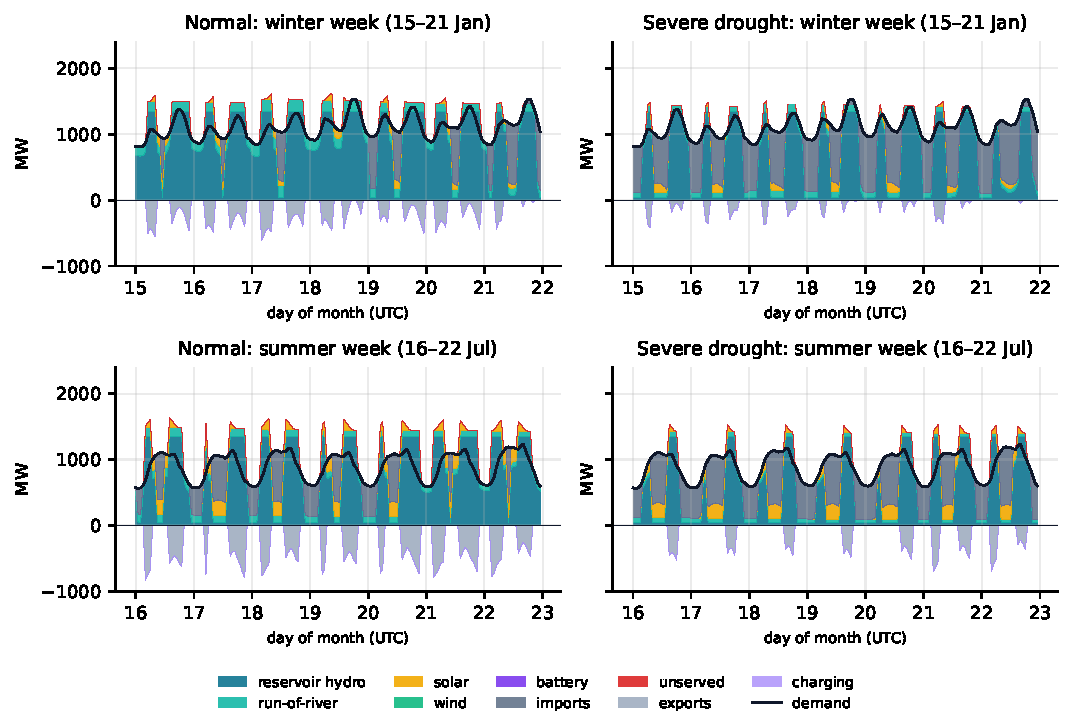
\includegraphics[width=\textwidth]{fig04_dispatch_normal_vs_drought.pdf}
\caption{Hourly dispatch in a winter and a summer week under normal conditions and severe drought (existing
fleet, full-year optimisation). Exports and battery charging are drawn below zero. In drought the reservoir
covers fewer hours and imports fill the evening peaks.}
\label{fig:dispatch}
\end{figure}

\begin{figure}[htbp]
\centering
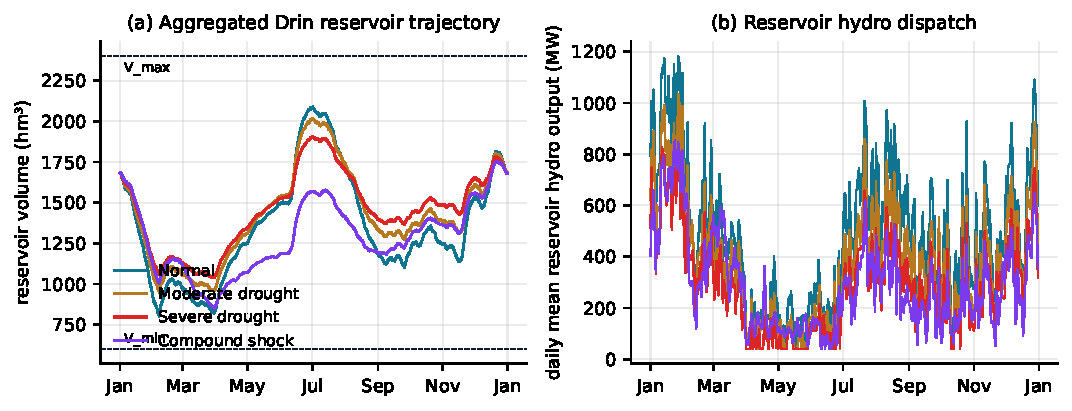
\includegraphics[width=\textwidth]{fig05_reservoir.pdf}
\caption{(a) Volume trajectory of the aggregated Drin reservoir and (b) daily reservoir hydro output under the
four presets (full-year hourly optimisation with $V_T=V_0$). The minimum operating volume is not reached in any
preset. Drought lowers releases rather than draining the reservoir, because the cyclic terminal condition
forces the deficit to be covered by imports.}
\label{fig:reservoir}
\end{figure}

\begin{table}[htbp]
\centering
\footnotesize
\caption{Annual hourly dispatch (8760 h, reference weather year). Energies in TWh, ENS in MWh, operating cost (imports $-$ exports + penalties + variable O\&M) in MEUR/yr, mean shadow price in EUR/MWh. Existing fleet unless stated.}
\label{tab:annual}
\begin{adjustbox}{max width=\linewidth}
\begin{tabular}{lrrrrrrrr}
\toprule
Case & Demand & Hydro & PV+wind & Imports & Exports & ENS & Opex & Price \\
\midrule
Normal & 8.00 & 6.77 & 0.46 & 2.00 & 1.23 & 0 & 40.8 & 97.2 \\
Moderate drought & 8.00 & 5.28 & 0.46 & 2.91 & 0.66 & 0 & 192.7 & 99.9 \\
Severe drought & 8.00 & 4.06 & 0.46 & 3.79 & 0.32 & 0 & 324.5 & 102.2 \\
Compound shock & 8.64 & 4.06 & 0.46 & 4.20 & 0.09 & 0 & 727.1 & 209.3 \\
Coordinated fleet, normal & 8.00 & 6.77 & 2.28 & 1.22 & 2.20 & 0 & -133.1 & 93.5 \\
Coordinated fleet, severe & 8.00 & 4.06 & 2.28 & 2.63 & 0.90 & 0 & 139.4 & 99.4 \\
\bottomrule
\end{tabular}
\end{adjustbox}
\end{table}


\subsection{Where reliability fails: interconnector availability and demand growth (Experiments F, G)}
A uniform import-price shock leaves dispatch unchanged, because relative prices stay the same. Annual cost
then rises linearly, from 324.5~MEUR at 1$\times$ to 968.4~MEUR at 3$\times$ (severe drought), with zero
unserved energy (Table~\ref{tab:exp-F}). Shortage appears only when import \emph{availability} falls. Under
severe drought with 8\% demand growth, availability of 75\% still serves all demand. At 50\%, 311~GWh are
unserved over 999~h with a peak shortfall of 811~MW. At 35\% and 25\% availability, unserved energy rises
to 1.40 and 2.16~TWh. These shortages are \emph{energy}-limited, not power-limited. With 50\% availability the
annual supply that can be delivered (hydro + PV + 450~MW of imports $\times$ 8{,}760~h) falls short of demand.
Consistent with this, a 400~MW / 1{,}600~MWh battery reduces unserved energy at 50\% availability by only 13\%
(311 to 270~GWh). At VOLL = 5{,}000~EUR/MWh even this partial reduction lowers annual cost by 199.8~MEUR,
well above the battery's 51.7~MEUR/yr annualised cost. At 35\% and 25\% availability the reduction is
1--2\% and the saving 97 and 59~MEUR/yr. Demand growth shows the same threshold behaviour (Table~\ref{tab:exp-G},
Fig.~\ref{fig:imports}c). With full interconnector availability, demand growth of up to 30\% is absorbed by
imports. With 50\% availability, unserved energy is 0, 456, 1{,}201 and 1{,}969~GWh at growth of 0, 10, 20 and
30\%, so loss-of-load hours rise from 0 to 4{,}088. In this model, therefore, the reliability of a
hydro-dependent system in drought is governed mainly by the availability of interconnection. This matters
because regional droughts can depress neighbours' export capacity at the same time.

\begin{table}[htbp]
\centering
\footnotesize
\caption{Experiment F: import price shocks and interconnector derating under severe drought (annual, hourly).}
\label{tab:exp-F}
\begin{tabular}{lrrrrr}
\toprule
Case (severe drought) & Imports (TWh) & Net imp. (TWh) & LOLH (h) & ENS (MWh) & Cost (MEUR/yr) \\
\midrule
Import price ×1.0 & 3.79 & 3.48 & 0 & 0 & 324.5 \\
Import price ×1.5 & 3.79 & 3.48 & 0 & 0 & 485.5 \\
Import price ×2.0 & 3.79 & 3.48 & 0 & 0 & 646.5 \\
Import price ×2.5 & 3.79 & 3.48 & 0 & 0 & 807.4 \\
Import price ×3.0 & 3.79 & 3.48 & 0 & 0 & 968.4 \\
NTC avail. 100%, +8\% demand & 4.33 & 4.12 & 0 & 0 & 391.7 \\
NTC avail. 75%, +8\% demand & 4.24 & 4.12 & 0 & 0 & 400.7 \\
NTC avail. 50%, +8\% demand & 3.81 & 3.81 & 999 & 310\,714 & 1\,957.2 \\
NTC avail. 35%, +8\% demand & 2.71 & 2.71 & 3\,391 & 1\,401\,990 & 7\,298.1 \\
NTC avail. 25%, +8\% demand & 1.95 & 1.95 & 4\,310 & 2\,162\,994 & 11\,022.9 \\
NTC 50%, +8\% dem., battery 400/1600 & 3.86 & 3.86 & 816 & 270\,120 & 1\,757.4 \\
NTC 35%, +8\% dem., battery 400/1600 & 2.74 & 2.74 & 3\,293 & 1\,382\,198 & 7\,200.9 \\
NTC 25%, +8\% dem., battery 400/1600 & 1.97 & 1.97 & 4\,267 & 2\,151\,012 & 10\,964.1 \\
\bottomrule
\end{tabular}
\end{table}


\subsection{Solar, storage and coordination (Experiments C, D, E)}
\paragraph{Solar without storage.} Adding PV reduces gross imports with diminishing returns
(Table~\ref{tab:exp-C}). Under normal conditions the reduction per added MW is 1{,}074, 898 and 699~MWh/MW
for +500, +1{,}000 and +1{,}500~MW. Under severe drought it is larger (1{,}406, 1{,}253 and 1{,}022~MWh/MW),
because a drier system exports less and imports more at the margin. Operating savings fall only slightly per
MW (138 to 131~kEUR/MW-yr in the normal year), because surplus midday PV can still be exported at 85\% of the
import price. Curtailment therefore stays small: at most 21~GWh, at +1{,}500~MW in the normal year. This
result rests on the assumed export capacity and price ratio (Section~\ref{sec:sensitivity}). The annualised
cost of PV is 80~kEUR/MW-yr, so under these assumptions every tested PV addition reduces total cost.

\paragraph{Batteries without new renewables.} A battery earns only intra-day arbitrage. The annual operating
savings are 5.5, 9.8 and 13.8~MEUR (normal) and 7.0, 12.7 and 17.9~MEUR (severe drought) for
200/800, 400/1{,}600 and 800/3{,}200~MW/MWh. Their annualised costs are 25.8, 51.7 and 103.3~MEUR/yr, so
arbitrage alone does not recover them. The value per unit is higher in drought, because the import price, not
the cheap reservoir, sets the marginal cost in more hours. Batteries also \emph{increase} gross imports: by
0.23--0.60~TWh in the normal year and similar amounts in the severe-drought year. They do this by storing
low-price imports for high-price hours. ``Reducing imports'' and ``reducing cost'' are therefore different
objectives for storage.

\paragraph{Coordination.} Combining PV (+1{,}000~MW) with a 400~MW / 1{,}600~MWh battery saves 146.9~MEUR/yr
in the normal year. That is 1.75~MEUR more than the sum of the separate savings (135.4 + 9.8). In severe
drought the corresponding synergy is 1.82~MEUR (Table~\ref{tab:exp-E}). The synergy is positive but small,
because an export route and the reservoir already absorb most PV surplus. The battery removes the remaining
2.2~GWh of PV curtailment.

\IfFileExists{tables/tab_exp_C.tex}{\begin{table}[htbp]
\centering
\footnotesize
\caption{Experiment C: PV additions without storage (annual, hourly).}
\label{tab:exp-C}
\begin{tabular}{lrrrrrr}
\toprule
Case & Imports (TWh) & Net imp. (TWh) & Curtail. (GWh) & Batt. cycles & ENS (MWh) & Opex (MEUR/yr) \\
\midrule
Normal, PV 300 MW & 2.00 & 0.77 & 0.0 & 0.0 & 0 & 40.8 \\
Normal, PV 800 MW & 1.46 & 0.00 & 0.0 & 0.0 & 0 & -28.3 \\
Normal, PV 1300 MW & 1.10 & -0.76 & 2.2 & 0.0 & 0 & -94.6 \\
Normal, PV 1800 MW & 0.95 & -1.51 & 20.7 & 0.0 & 0 & -156.3 \\
Severe, PV 300 MW & 3.79 & 3.48 & 0.0 & 0.0 & 0 & 324.5 \\
Severe, PV 800 MW & 3.09 & 2.71 & 0.0 & 0.0 & 0 & 252.7 \\
Severe, PV 1300 MW & 2.54 & 1.94 & 0.0 & 0.0 & 0 & 182.8 \\
Severe, PV 1800 MW & 2.26 & 1.18 & 2.3 & 0.0 & 0 & 117.0 \\
\bottomrule
\end{tabular}
\end{table}
}{}
\IfFileExists{tables/tab_exp_E.tex}{\begin{table}[htbp]
\centering
\footnotesize
\caption{Experiment E: coordinated portfolios (fixed fleets, annual hourly dispatch). Battery = 400 MW / 1600 MWh.}
\label{tab:exp-E}
\begin{adjustbox}{max width=\linewidth}
\begin{tabular}{lrrrrrr}
\toprule
Case & Imports (TWh) & Net imp. (TWh) & Curtail. (GWh) & Batt. cycles & ENS (MWh) & Opex (MEUR/yr) \\
\midrule
Normal, baseline & 2.00 & 0.77 & 0.0 & 0.0 & 0 & 40.8 \\
Normal, pv+1000 & 1.10 & -0.76 & 2.2 & 0.0 & 0 & -94.6 \\
Normal, batt400/1600 & 2.42 & 0.84 & 0.0 & 401.4 & 0 & 31.0 \\
Normal, pv+1000\&batt & 1.35 & -0.70 & 0.0 & 390.0 & 0 & -106.2 \\
Normal, pv+1000\&wind300 & 0.99 & -1.05 & 2.8 & 0.0 & 0 & -121.7 \\
Normal, pv+1000\&wind300\&batt & 1.22 & -0.99 & 0.0 & 385.1 & 0 & -133.1 \\
Severe, baseline & 3.79 & 3.48 & 0.0 & 0.0 & 0 & 324.5 \\
Severe, pv+1000 & 2.54 & 1.94 & 0.0 & 0.0 & 0 & 182.8 \\
Severe, batt400/1600 & 4.20 & 3.56 & 0.0 & 463.8 & 0 & 311.8 \\
Severe, pv+1000\&batt & 2.84 & 2.02 & 0.0 & 470.3 & 0 & 168.3 \\
Severe, pv+1000\&wind300 & 2.34 & 1.66 & 0.0 & 0.0 & 0 & 153.8 \\
Severe, pv+1000\&wind300\&batt & 2.63 & 1.74 & 0.0 & 468.5 & 0 & 139.4 \\
\bottomrule
\end{tabular}
\end{adjustbox}
\end{table}
}{}

\begin{figure}[htbp]
\centering
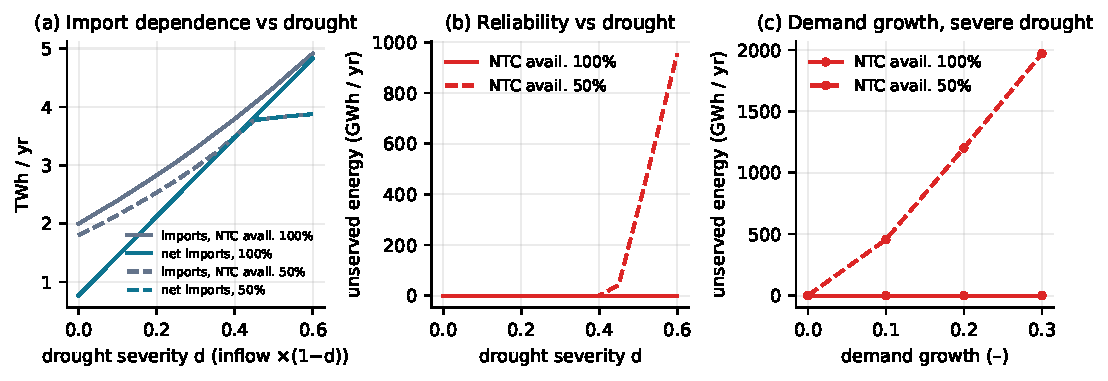
\includegraphics[width=\textwidth]{fig07_imports_reliability.pdf}
\caption{(a) Gross and net imports and (b) unserved energy as functions of drought severity $d$ (inflows scaled by
$1-d$, existing fleet) with full (solid) and halved (dashed) interconnector availability. (c) Unserved energy
under severe drought as demand grows. Shortage appears only when transfer availability is restricted.}
\label{fig:imports}
\end{figure}

\begin{figure}[htbp]
\centering
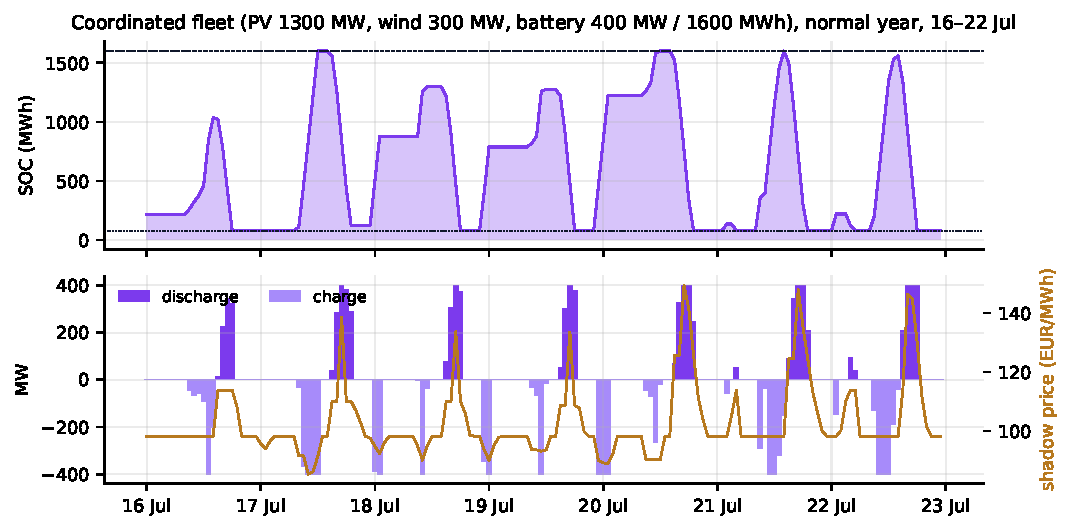
\includegraphics[width=\textwidth]{fig06_battery_soc.pdf}
\caption{Battery operation in a summer week (coordinated fleet: PV 1{,}300~MW, wind 300~MW, battery 400~MW /
1{,}600~MWh). The battery charges around midday when PV depresses the shadow price and discharges in the
evening peak: roughly one cycle per day (385 equivalent full cycles per year).}
\label{fig:battery}
\end{figure}

\subsection{Marginal value of flexibility (Experiment J)}
Table~\ref{tab:marginal} and Fig.~\ref{fig:marginal} report finite-difference and dual-based marginal values
around a base fleet with PV 300~MW, a 200~MW / 800~MWh battery and 900~MW of import capacity. In every
non-degenerate case the dual lies within the finite-difference interval $[\Delta^+,\Delta^-]$, as LP theory
predicts. Four results stand out:
\begin{itemize}
\item \textbf{PV} has an operating value of 140~kEUR/MW-yr (normal), 146 (severe drought) and 314 (compound
shock), against an annualised cost of 80~kEUR/MW-yr.
\item \textbf{Wind} (CF $\approx$ 0.11 from coarse reanalysis) is worth 93--99~kEUR/MW-yr against 133~kEUR/MW-yr
in normal and drought years, and 202 under the compound shock. The wind dual at zero capacity is flagged as a
degenerate corner, and the right finite difference is reported instead.
\item \textbf{Battery power and energy are not substitutes.} With 800~MWh installed, an extra MW of discharge
power is worth 12.7--15.5~kEUR/yr in normal and drought years, above its 10.1~kEUR/yr annualised cost.
An extra MWh is worth only 2.3--4.1~kEUR/yr, against 29.8. Shorter-duration batteries are therefore closer
to break-even than the 4-hour configuration.
\item \textbf{Import capacity} is worth 2~kEUR/MW-yr in a normal year, 9 in severe drought and 175 under the
compound shock. This is the largest increase of any resource, and it confirms that interconnection is the
critical flexibility resource under compound stress. Additional reservoir \emph{volume} has zero marginal value
in all cases: the volume bound never binds, and the energy limit comes from inflow rather than storage size.
\end{itemize}

\begin{table}[htbp]
\centering
\footnotesize
\caption{Marginal operating value of flexibility (kEUR per unit per year) around the base fleet (PV 300 MW, battery 200 MW/800 MWh, NTC 900 MW, $V^{\max}$ 2400 hm$^3$). $\Delta^+$: value of adding the next increment; $\Delta^-$: value of the last increment. Ann. cost: annualised cost of one more unit.}
\label{tab:marginal}
\begin{adjustbox}{max width=\linewidth}
\begin{tabular}{lrrrrrrr}
\toprule
Resource & Scenario & Unit & $\Delta^+$ & $\Delta^-$ & Dual & Dual valid & Ann. cost \\
\midrule
battery energy & normal & MWh & 2.3 & 3.0 & 2.6 & yes & 29.8 \\
battery power & normal & MW & 12.7 & 16.2 & 14.5 & yes & 10.1 \\
solar pv & normal & MW & 139.7 & 140.0 & 139.8 & yes & 80.1 \\
wind & normal & MW & 92.8 & -- & 92.9 & no & 132.7 \\
import capacity & normal & MW & 1.7 & 2.7 & 2.1 & yes & 30.0 \\
reservoir volume & normal & hm$^3$ & 0.0 & 0.0 & 0.0 & yes & -- \\
battery energy & severe drought & MWh & 3.1 & 4.1 & 3.3 & yes & 29.8 \\
battery power & severe drought & MW & 15.5 & 20.3 & 18.6 & yes & 10.1 \\
solar pv & severe drought & MW & 145.6 & 146.1 & 145.8 & yes & 80.1 \\
wind & severe drought & MW & 99.2 & -- & 99.3 & no & 132.7 \\
import capacity & severe drought & MW & 7.5 & 11.2 & 9.3 & yes & 30.0 \\
reservoir volume & severe drought & hm$^3$ & 0.0 & 0.0 & 0.0 & yes & -- \\
battery energy & compound shock & MWh & 4.1 & 5.4 & 4.6 & yes & 29.8 \\
battery power & compound shock & MW & 8.2 & 11.7 & 10.0 & yes & 10.1 \\
solar pv & compound shock & MW & 314.2 & 322.1 & 318.1 & yes & 80.1 \\
wind & compound shock & MW & 201.8 & -- & 202.5 & no & 132.7 \\
import capacity & compound shock & MW & 153.5 & 197.4 & 174.5 & yes & 30.0 \\
reservoir volume & compound shock & hm$^3$ & 0.0 & 0.0 & 0.0 & yes & -- \\
\bottomrule
\end{tabular}
\end{adjustbox}
\end{table}


\begin{figure}[htbp]
\centering
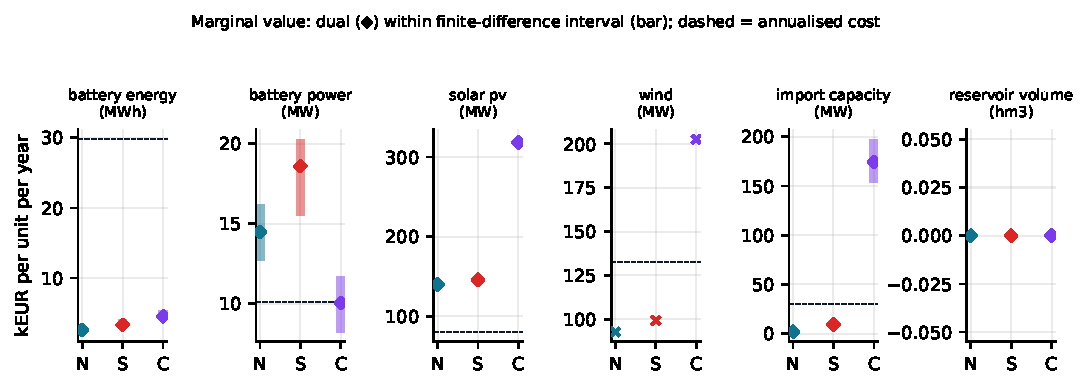
\includegraphics[width=\textwidth]{fig11_marginal_value.pdf}
\caption{Marginal operating value of each flexibility resource in the normal (N), severe-drought (S) and
compound-shock (C) cases. Bars show the finite-difference interval $[\Delta^+,\Delta^-]$, diamonds the dual
value (crosses mark degenerate corners), and the dashed line the annualised cost of one more unit.}
\label{fig:marginal}
\end{figure}

\subsection{Budget-constrained investment (Experiment H)}
For the normal year, the deterministic optimum spends every budget level from 100 to 1{,}500~MEUR entirely on
PV: 126, 315, 629, 944, 1{,}258 and 1{,}888~MW. At 2{,}000~MEUR the PV bound (+2{,}000~MW) binds and the
budget does not. Neither wind nor storage enters at any budget. The budget shadow price falls from 0.070 to
0.024~EUR of annual saving per euro of capital as PV grows. These are diminishing but still positive returns,
and they are consistent with the PV marginal value of Experiment~J (140~kEUR/MW-yr against 80~kEUR/MW-yr of
annualised cost). The result reflects three assumptions: exports absorb midday surplus at 85\% of the import
price, there is no reserve requirement, and wind capacity factors are about 0.11 from coarse reanalysis.
Section~\ref{sec:sensitivity} tests the first of these.

\subsection{Deterministic versus stochastic planning (Experiment I)}
The two-stage programme has five scenarios, eight hourly weeks each, a 500~MEUR budget and CVaR at $\alpha=0.9$.
For every risk weight tested ($\lambda\in\{0,0.25,1,4\}$) it selects the \emph{same} portfolio as the
deterministic normal-year plan: +629~MW of PV, with no wind and no storage (Table~\ref{tab:risk-sweep}). The same
holds at a 1{,}500~MEUR budget. Each wait-and-see problem also chooses this plan, so the value of the stochastic
solution and the expected value of perfect information are both zero to solver precision
(Table~\ref{tab:stochastic}). CVaR$_{0.9}$ of operating cost is 397~MEUR/yr for both plans. Hypothesis~I is
therefore \textbf{not supported} under the base assumptions. PV is a \emph{no-regret} investment in every
scenario. Its value is set mainly by the import price, and it rises under stress. The budget binds before any
resource whose value depends on the scenario becomes competitive. The stochastic machinery still answers
question~6 of the study: under these assumptions, deterministic planning for an average year is not
penalised. One qualification matters. None of the five planning scenarios, the compound shock included
(70\% availability), reaches the import-availability regime of $\le$50\% in which shortages occur and
batteries become valuable (Sections~\ref{sec:results} and~\ref{sec:sensitivity}). A scenario set with even a
small probability of that regime could change the plan, and this is a priority for future work.

\IfFileExists{tables/tab_stochastic.tex}{\begin{table}[htbp]
\centering
\small
\caption{Two-stage stochastic versus deterministic planning (budget 500 MEUR, 8 representative weeks, water-value boundaries). E[cost]: expected total annualised cost (MEUR/yr) on all five scenarios; CVaR of operating cost (MEUR/yr). Risk-adjusted VSS = 0.00 MEUR/yr; EVPI is reported only for $\lambda=0$.}
\label{tab:stochastic}
\begin{adjustbox}{max width=\linewidth}
\begin{tabular}{lrrrrrr}
\toprule
Plan & +PV & +Wind & +B MW & +B MWh & E[cost] & CVaR$_{0.9}$ \\
\midrule
Stochastic (RP), $\lambda$=1 & 629 & 0 & 0 & 0 & 70.9 & 397.3 \\
Deterministic (normal year) & 629 & 0 & 0 & 0 & 70.9 & 397.3 \\
\bottomrule
\end{tabular}
\end{adjustbox}
\end{table}
}{}

\subsection{When does stochastic planning matter? (Experiment I2)}
To find the conditions under which uncertainty changes the decision, we repeated the comparison with export
capacity limited to 300~MW. Surplus PV must then be stored, absorbed by the reservoir or curtailed. We also
raised the budget, so that PV saturates before the budget binds (Table~\ref{tab:i2}). With 900~MW of export
capacity the stochastic and deterministic plans remain identical at every risk weight (VSS = 0). With
restricted exports and risk-neutral planning ($\lambda=0$), the stochastic plan adds slightly more PV than the
deterministic one (+26~MW at 1{,}000~MEUR, +75~MW at 1{,}500~MEUR), and the VSS is only 0.2--0.3~MEUR/yr. With
restricted exports, a 1{,}500~MEUR budget and $\lambda=1$, the decision changes qualitatively. The risk-averse
plan adds 1{,}520~MW of PV, 230~MW of \emph{wind} and a 30~MW / 66~MWh battery. The deterministic plan adds
1{,}232~MW of PV only. In the representative-week model the risk-averse plan raises expected cost by
7.8~MEUR/yr and lowers CVaR$_{0.9}$ of operating cost by 79~MEUR/yr (from 292 to 213); the risk-adjusted VSS is
71.5~MEUR/yr. Full-year chronological re-evaluation of the two plans confirms the trade-off. Expected total
cost is higher by 15.1~MEUR/yr (74.6 vs 59.5), CVaR$_{0.9}$ of operating cost is lower by 74.5~MEUR/yr (208.2
vs 282.7), and neither plan has any unserved energy. The hedge is mainly wind rather than storage. Once PV saturates
under the export limit, wind is the cheapest remaining way to cut imports in the high-price stress scenarios.
We did not decompose this mechanism further, for example by wind--PV correlation or season. Stochastic, risk-aware planning therefore matters when a no-regret resource
saturates because its surplus cannot leave the system. In that regime the choice among the remaining resources
depends on the tail scenarios.

\IfFileExists{tables/tab_i2.tex}{\begin{table}[htbp]
\centering
\scriptsize
\caption{Experiment I2: stochastic (RP) versus deterministic-plan evaluation (EEV) under restricted and full export capacity. Additions as PV/wind MW / battery MW/MWh; E = expected total annualised cost, CVaR$_{0.9}$ of operating cost and risk-adjusted VSS in MEUR/yr (representative weeks, water-value boundaries).}
\label{tab:i2}
\begin{adjustbox}{max width=\linewidth}
\begin{tabular}{lrrrrrrrrr}
\toprule
Export MW & Budget & $\lambda$ & Stoch. adds & Det. adds & E RP & E EEV & CVaR RP & CVaR EEV & VSS \\
\midrule
300 & 1\,000 & 0 & 1\,258/0/0/0 & 1\,232/0/0/0 & 62.0 & 62.1 & 288.1 & 292.0 & 0.2 \\
300 & 1\,000 & 1 & 1\,258/0/0/0 & 1\,232/0/0/0 & 62.0 & 62.1 & 288.1 & 292.0 & 4.1 \\
300 & 1\,500 & 0 & 1\,307/0/0/0 & 1\,232/0/0/0 & 61.8 & 62.1 & 281.1 & 292.0 & 0.3 \\
300 & 1\,500 & 1 & 1\,520/230/30/66 & 1\,232/0/0/0 & 70.0 & 62.1 & 212.7 & 292.0 & 71.5 \\
900 & 1\,500 & 0 & 1\,888/0/0/0 & 1\,888/0/0/0 & 12.9 & 12.9 & 170.2 & 170.2 & 0.0 \\
900 & 1\,500 & 1 & 1\,888/0/0/0 & 1\,888/0/0/0 & 12.9 & 12.9 & 170.2 & 170.2 & 0.0 \\
\bottomrule
\end{tabular}
\end{adjustbox}
\end{table}
}{}

\begin{figure}[htbp]
\centering
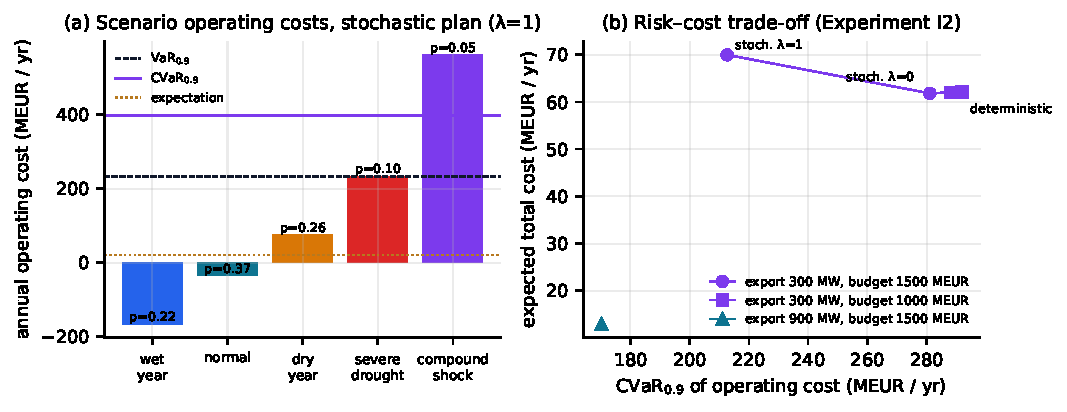
\includegraphics[width=\textwidth]{fig09_cvar.pdf}
\caption{(a) Annualised operating cost of the reference stochastic plan in each scenario, with probabilities, VaR$_{0.9}$,
CVaR$_{0.9}$ and the expectation. In the base case this plan is identical to the deterministic plan. (b) Expected total cost
versus CVaR$_{0.9}$ of operating cost for the deterministic plan and the stochastic plans ($\lambda=0,1$) in
Experiment~I2. Only with restricted exports and a large budget does risk aversion buy a material reduction in tail
cost.}
\label{fig:cvar}
\end{figure}


\subsection{Investment frontier}
Figure~\ref{fig:frontier} and Table~\ref{tab:strategies} compare the required strategies, the budget sweep and
the stochastic plans on equal terms, using the same representative-week evaluation. At 500~MEUR the strategies
rank as follows by expected total annualised cost: solar (70.9~MEUR/yr; identical to the coordinated and
climate-robust optima), baseline (109.4), wind (112.1) and battery-only (164.9). The battery-only plan has the
highest cost and the highest imports, because arbitrage increases gross imports. Across budgets, larger PV
additions lower both expected cost and imports. The non-dominated set in (expected cost, expected imports)
therefore collapses to the largest-PV plan, and the trade-off appears only in capital spent versus imports
(\texttt{pareto\_capex\_imports} in the artefact). We report this degenerate frontier as it is, rather than
constructing an artificial trade-off.

\begin{figure}[htbp]
\centering
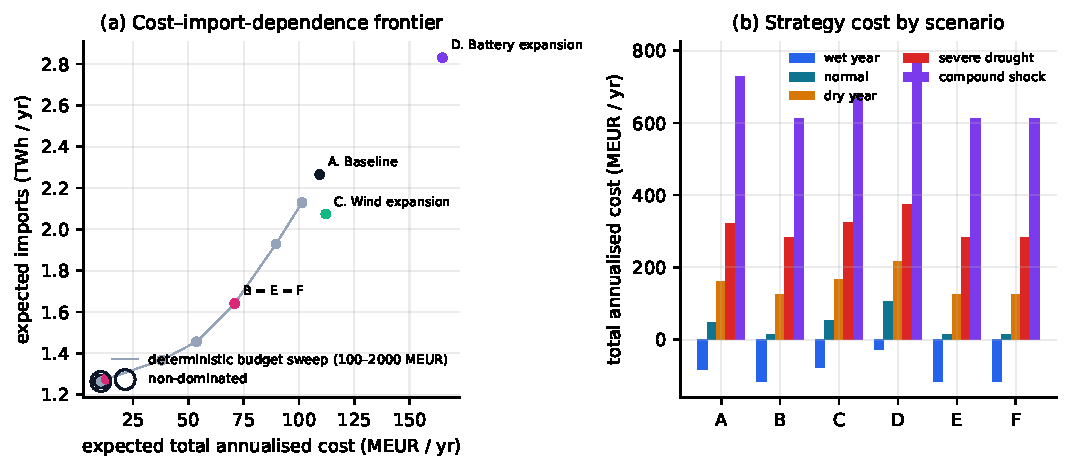
\includegraphics[width=\textwidth]{fig08_investment_frontier.pdf}
\caption{(a) Strategies in the plane of expected total annualised cost and expected imports, evaluated with the
same representative-week model over five scenarios. Outlined points are non-dominated. (b) Total annualised cost
of the required strategies A--F in each scenario.}
\label{fig:frontier}
\end{figure}

\begin{table}[htbp]
\centering
\scriptsize
\caption{Investment strategies evaluated on the five-scenario set (representative weeks, hourly). Additions in MW/MWh, overnight capex in MEUR, expected total annualised cost and severe-drought cost in MEUR/yr, expected imports in TWh/yr; ND marks the non-dominated set in (expected cost, expected imports).}
\label{tab:strategies}
\begin{tabular}{p{4.2cm}rrrrrrrrc}
\toprule
Strategy & +PV & +Wind & +B MW & +B MWh & Capex & E[cost] & E[imp.] & Cost sev. & ND \\
\midrule
A. Baseline & 0 & 0 & 0 & 0 & 0 & 109.4 & 2.27 & 320.4 &  \\
B. Solar expansion & 629 & 0 & 0 & 0 & 500 & 70.9 & 1.64 & 283.5 &  \\
C. Wind expansion & 0 & 418 & 0 & 0 & 500 & 112.1 & 2.07 & 323.7 &  \\
D. Battery expansion & 0 & 0 & 522 & 2\,087 & 500 & 164.9 & 2.83 & 373.4 &  \\
E. Coordinated (deterministic optimum) & 629 & 0 & 0 & 0 & 500 & 70.9 & 1.64 & 283.5 &  \\
F. Climate-robust (stochastic, CVaR λ=1) & 629 & 0 & 0 & 0 & 500 & 70.9 & 1.64 & 283.5 &  \\
Budget 100 MEUR (det.) & 126 & 0 & 0 & 0 & 100 & 101.4 & 2.13 & 312.9 &  \\
Budget 250 MEUR (det.) & 315 & 0 & 0 & 0 & 250 & 89.7 & 1.93 & 301.8 &  \\
Budget 750 MEUR (det.) & 944 & 0 & 0 & 0 & 750 & 53.7 & 1.46 & 266.5 &  \\
Budget 1000 MEUR (det.) & 1\,258 & 0 & 0 & 0 & 1\,000 & 37.9 & 1.37 & 251.2 &  \\
Budget 1500 MEUR (det.) & 1\,888 & 0 & 0 & 0 & 1\,500 & 12.9 & 1.27 & 225.1 &  \\
Budget 2000 MEUR (det.) & 2\,000 & 0 & 0 & 0 & 1\,589 & 10.4 & 1.26 & 222.3 & $\bullet$ \\
Stochastic λ=0.0 (500 MEUR) & 629 & 0 & 0 & 0 & 500 & 70.9 & 1.64 & 283.5 &  \\
Stochastic λ=0.25 (500 MEUR) & 629 & 0 & 0 & 0 & 500 & 70.9 & 1.64 & 283.5 &  \\
Stochastic λ=4.0 (500 MEUR) & 629 & 0 & 0 & 0 & 500 & 70.9 & 1.64 & 283.5 &  \\
Stochastic λ=0.0 (1500 MEUR) & 1\,888 & 0 & 0 & 0 & 1\,500 & 12.9 & 1.27 & 225.1 &  \\
Stochastic λ=4.0 (1500 MEUR) & 1\,888 & 0 & 0 & 0 & 1\,500 & 12.9 & 1.27 & 225.1 &  \\
\bottomrule
\end{tabular}
\end{table}


\subsection{Validity of the representative-week approximation}
\label{sec:chrono}
Seven plans were re-evaluated with full-year chronological hourly dispatch on all five scenarios. With the
water-value boundary, the representative-week model's expected total cost differs from chronology by 1.7 to
10.0~MEUR/yr in absolute terms. It overstates the cost of the PV plans by 4.2--8.7~MEUR/yr and understates the
wind plan by 10.0~MEUR/yr. Both models find no unserved energy for any plan, and the strategies rank in the
same order (ties between identical plans aside). An earlier variant pinned each week's terminal volume
($V_T\ge\bar V^T$). That variant overstated cost by up to 20.4~MEUR/yr and produced spurious shortages in the
sampled drought weeks. Those shortages made a PV--battery portfolio look better on tail risk, but full
chronology showed this to be an artefact: the PV-only plan had lower expected cost (66.7 vs 76.3~MEUR/yr) and
lower CVaR (443.5 vs 455.7~MEUR/yr). We report this as a methodological finding. How the seasonal boundary of a
representative period is treated can change the investment recommendation, and validation against full
chronology should be routine.

\IfFileExists{tables/tab_chrono.tex}{\begin{table}[htbp]
\centering
\footnotesize
\caption{Full-year chronological (8760 h, hourly) versus representative-week (8 weeks, water-value boundaries) evaluation of the same plans on the five-scenario set. Costs in MEUR/yr; CVaR$_{0.9}$ of total annualised cost; ENS expected MWh/yr.}
\label{tab:chrono}
\begin{adjustbox}{max width=\linewidth}
\begin{tabular}{p{5cm}rrrrrr}
\toprule
Plan & E[cost] chrono & E[cost] rep. & Diff. & CVaR chrono & CVaR rep. & ENS chrono \\
\midrule
A. Baseline & 107.7 & 109.4 & 1.7 & 525.8 & 524.0 & 0 \\
B. Solar expansion & 66.7 & 70.9 & 4.2 & 443.5 & 447.7 & 0 \\
C. Wind expansion & 122.1 & 112.1 & -10.0 & 520.0 & 502.9 & 0 \\
D. Battery expansion & 162.8 & 164.9 & 2.1 & 577.9 & 576.9 & 0 \\
F. Climate-robust (stochastic, CVaR λ=1) & 66.7 & 70.9 & 4.2 & 443.5 & 447.7 & 0 \\
Budget 1500 MEUR (det.) & 4.2 & 12.9 & 8.7 & 308.6 & 321.4 & 0 \\
Stochastic λ=0.0 (500 MEUR) & 66.7 & 70.9 & 4.2 & 443.5 & 447.7 & 0 \\
\bottomrule
\end{tabular}
\end{adjustbox}
\end{table}
}{}

